% Created by tikzDevice version 0.12.3 on 2020-01-08 13:37:55
% !TEX encoding = UTF-8 Unicode
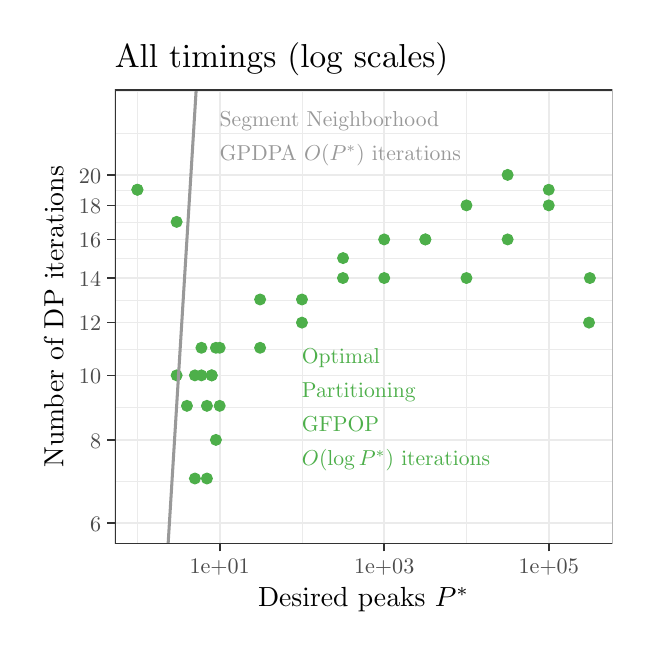
\begin{tikzpicture}[x=1pt,y=1pt]
\definecolor{fillColor}{RGB}{255,255,255}
\path[use as bounding box,fill=fillColor,fill opacity=0.00] (0,0) rectangle (216.81,216.81);
\begin{scope}
\path[clip] (  0.00,  0.00) rectangle (216.81,216.81);
\definecolor{drawColor}{RGB}{255,255,255}
\definecolor{fillColor}{RGB}{255,255,255}

\path[draw=drawColor,line width= 0.6pt,line join=round,line cap=round,fill=fillColor] (  0.00,  0.00) rectangle (216.81,216.81);
\end{scope}
\begin{scope}
\path[clip] ( 31.48, 30.33) rectangle (211.31,194.39);
\definecolor{fillColor}{RGB}{255,255,255}

\path[fill=fillColor] ( 31.48, 30.33) rectangle (211.31,194.39);
\definecolor{drawColor}{gray}{0.92}

\path[draw=drawColor,line width= 0.3pt,line join=round] ( 31.48, 52.82) --
	(211.31, 52.82);

\path[draw=drawColor,line width= 0.3pt,line join=round] ( 31.48, 79.51) --
	(211.31, 79.51);

\path[draw=drawColor,line width= 0.3pt,line join=round] ( 31.48,100.70) --
	(211.31,100.70);

\path[draw=drawColor,line width= 0.3pt,line join=round] ( 31.48,118.28) --
	(211.31,118.28);

\path[draw=drawColor,line width= 0.3pt,line join=round] ( 31.48,133.31) --
	(211.31,133.31);

\path[draw=drawColor,line width= 0.3pt,line join=round] ( 31.48,146.45) --
	(211.31,146.45);

\path[draw=drawColor,line width= 0.3pt,line join=round] ( 31.48,158.11) --
	(211.31,158.11);

\path[draw=drawColor,line width= 0.3pt,line join=round] ( 31.48,178.65) --
	(211.31,178.65);

\path[draw=drawColor,line width= 0.3pt,line join=round] ( 31.48,193.68) --
	(211.31,193.68);

\path[draw=drawColor,line width= 0.3pt,line join=round] ( 39.65, 30.33) --
	( 39.65,194.39);

\path[draw=drawColor,line width= 0.3pt,line join=round] ( 99.11, 30.33) --
	( 99.11,194.39);

\path[draw=drawColor,line width= 0.3pt,line join=round] (158.56, 30.33) --
	(158.56,194.39);

\path[draw=drawColor,line width= 0.6pt,line join=round] ( 31.48, 37.79) --
	(211.31, 37.79);

\path[draw=drawColor,line width= 0.6pt,line join=round] ( 31.48, 67.85) --
	(211.31, 67.85);

\path[draw=drawColor,line width= 0.6pt,line join=round] ( 31.48, 91.17) --
	(211.31, 91.17);

\path[draw=drawColor,line width= 0.6pt,line join=round] ( 31.48,110.23) --
	(211.31,110.23);

\path[draw=drawColor,line width= 0.6pt,line join=round] ( 31.48,126.34) --
	(211.31,126.34);

\path[draw=drawColor,line width= 0.6pt,line join=round] ( 31.48,140.29) --
	(211.31,140.29);

\path[draw=drawColor,line width= 0.6pt,line join=round] ( 31.48,152.60) --
	(211.31,152.60);

\path[draw=drawColor,line width= 0.6pt,line join=round] ( 31.48,163.61) --
	(211.31,163.61);

\path[draw=drawColor,line width= 0.6pt,line join=round] ( 69.38, 30.33) --
	( 69.38,194.39);

\path[draw=drawColor,line width= 0.6pt,line join=round] (128.84, 30.33) --
	(128.84,194.39);

\path[draw=drawColor,line width= 0.6pt,line join=round] (188.29, 30.33) --
	(188.29,194.39);
\definecolor{drawColor}{RGB}{77,175,74}
\definecolor{fillColor}{RGB}{77,175,74}

\path[draw=drawColor,line width= 0.4pt,line join=round,line cap=round,fill=fillColor] ( 39.65,158.25) circle (  1.96);

\path[draw=drawColor,line width= 0.4pt,line join=round,line cap=round,fill=fillColor] ( 53.83, 91.17) circle (  1.96);

\path[draw=drawColor,line width= 0.4pt,line join=round,line cap=round,fill=fillColor] ( 57.55, 80.16) circle (  1.96);

\path[draw=drawColor,line width= 0.4pt,line join=round,line cap=round,fill=fillColor] ( 60.43, 91.17) circle (  1.96);

\path[draw=drawColor,line width= 0.4pt,line join=round,line cap=round,fill=fillColor] ( 62.78,101.13) circle (  1.96);

\path[draw=drawColor,line width= 0.4pt,line join=round,line cap=round,fill=fillColor] ( 64.77, 53.90) circle (  1.96);

\path[draw=drawColor,line width= 0.4pt,line join=round,line cap=round,fill=fillColor] ( 66.50, 91.17) circle (  1.96);

\path[draw=drawColor,line width= 0.4pt,line join=round,line cap=round,fill=fillColor] ( 68.02,101.13) circle (  1.96);

\path[draw=drawColor,line width= 0.4pt,line join=round,line cap=round,fill=fillColor] ( 69.38, 80.16) circle (  1.96);

\path[draw=drawColor,line width= 0.4pt,line join=round,line cap=round,fill=fillColor] ( 83.99,118.59) circle (  1.96);

\path[draw=drawColor,line width= 0.4pt,line join=round,line cap=round,fill=fillColor] ( 99.11,110.23) circle (  1.96);

\path[draw=drawColor,line width= 0.4pt,line join=round,line cap=round,fill=fillColor] (113.96,133.55) circle (  1.96);

\path[draw=drawColor,line width= 0.4pt,line join=round,line cap=round,fill=fillColor] (128.82,140.29) circle (  1.96);

\path[draw=drawColor,line width= 0.4pt,line join=round,line cap=round,fill=fillColor] (143.70,140.29) circle (  1.96);

\path[draw=drawColor,line width= 0.4pt,line join=round,line cap=round,fill=fillColor] (158.56,152.60) circle (  1.96);

\path[draw=drawColor,line width= 0.4pt,line join=round,line cap=round,fill=fillColor] (173.43,163.61) circle (  1.96);

\path[draw=drawColor,line width= 0.4pt,line join=round,line cap=round,fill=fillColor] (188.29,152.60) circle (  1.96);

\path[draw=drawColor,line width= 0.4pt,line join=round,line cap=round,fill=fillColor] (203.14,126.34) circle (  1.96);

\path[draw=drawColor,line width= 0.4pt,line join=round,line cap=round,fill=fillColor] ( 39.65,158.25) circle (  1.96);

\path[draw=drawColor,line width= 0.4pt,line join=round,line cap=round,fill=fillColor] ( 53.83,146.63) circle (  1.96);

\path[draw=drawColor,line width= 0.4pt,line join=round,line cap=round,fill=fillColor] ( 60.43, 53.90) circle (  1.96);

\path[draw=drawColor,line width= 0.4pt,line join=round,line cap=round,fill=fillColor] ( 62.78, 91.17) circle (  1.96);

\path[draw=drawColor,line width= 0.4pt,line join=round,line cap=round,fill=fillColor] ( 64.77, 80.16) circle (  1.96);

\path[draw=drawColor,line width= 0.4pt,line join=round,line cap=round,fill=fillColor] ( 66.50, 91.17) circle (  1.96);

\path[draw=drawColor,line width= 0.4pt,line join=round,line cap=round,fill=fillColor] ( 68.02, 67.85) circle (  1.96);

\path[draw=drawColor,line width= 0.4pt,line join=round,line cap=round,fill=fillColor] ( 69.38,101.13) circle (  1.96);

\path[draw=drawColor,line width= 0.4pt,line join=round,line cap=round,fill=fillColor] ( 83.99,101.13) circle (  1.96);

\path[draw=drawColor,line width= 0.4pt,line join=round,line cap=round,fill=fillColor] ( 99.11,118.59) circle (  1.96);

\path[draw=drawColor,line width= 0.4pt,line join=round,line cap=round,fill=fillColor] (113.92,126.34) circle (  1.96);

\path[draw=drawColor,line width= 0.4pt,line join=round,line cap=round,fill=fillColor] (128.84,126.34) circle (  1.96);

\path[draw=drawColor,line width= 0.4pt,line join=round,line cap=round,fill=fillColor] (143.70,140.29) circle (  1.96);

\path[draw=drawColor,line width= 0.4pt,line join=round,line cap=round,fill=fillColor] (158.56,126.34) circle (  1.96);

\path[draw=drawColor,line width= 0.4pt,line join=round,line cap=round,fill=fillColor] (173.43,140.29) circle (  1.96);

\path[draw=drawColor,line width= 0.4pt,line join=round,line cap=round,fill=fillColor] (188.29,158.25) circle (  1.96);

\path[draw=drawColor,line width= 0.4pt,line join=round,line cap=round,fill=fillColor] (202.84,110.23) circle (  1.96);
\definecolor{drawColor}{gray}{0.60}

\path[draw=drawColor,line width= 1.1pt,line join=round] ( 48.88,  0.00) -- ( 62.27,216.81);

\node[text=drawColor,anchor=base west,inner sep=0pt, outer sep=0pt, scale=  0.78] at ( 69.38,181.20) {Segment Neighborhood};

\node[text=drawColor,anchor=base west,inner sep=0pt, outer sep=0pt, scale=  0.78] at ( 69.38,168.91) {GPDPA $O(P^*)$ iterations};

\node[text=drawColor,anchor=base west,inner sep=0pt, outer sep=0pt, scale=  0.78] at ( 69.38,156.62) {};

\node[text=drawColor,anchor=base west,inner sep=0pt, outer sep=0pt, scale=  0.78] at ( 69.38,144.32) {};
\definecolor{drawColor}{RGB}{77,175,74}

\node[text=drawColor,anchor=base west,inner sep=0pt, outer sep=0pt, scale=  0.78] at ( 99.11, 95.40) {Optimal};

\node[text=drawColor,anchor=base west,inner sep=0pt, outer sep=0pt, scale=  0.78] at ( 99.11, 83.11) {Partitioning};

\node[text=drawColor,anchor=base west,inner sep=0pt, outer sep=0pt, scale=  0.78] at ( 99.11, 70.81) {GFPOP};

\node[text=drawColor,anchor=base west,inner sep=0pt, outer sep=0pt, scale=  0.78] at ( 99.11, 58.52) {$O(\log P^*)$ iterations};
\definecolor{drawColor}{gray}{0.20}

\path[draw=drawColor,line width= 0.6pt,line join=round,line cap=round] ( 31.48, 30.33) rectangle (211.31,194.39);
\end{scope}
\begin{scope}
\path[clip] (  0.00,  0.00) rectangle (216.81,216.81);
\definecolor{drawColor}{gray}{0.30}

\node[text=drawColor,anchor=base east,inner sep=0pt, outer sep=0pt, scale=  0.80] at ( 26.53, 34.83) {6};

\node[text=drawColor,anchor=base east,inner sep=0pt, outer sep=0pt, scale=  0.80] at ( 26.53, 64.89) {8};

\node[text=drawColor,anchor=base east,inner sep=0pt, outer sep=0pt, scale=  0.80] at ( 26.53, 88.22) {10};

\node[text=drawColor,anchor=base east,inner sep=0pt, outer sep=0pt, scale=  0.80] at ( 26.53,107.27) {12};

\node[text=drawColor,anchor=base east,inner sep=0pt, outer sep=0pt, scale=  0.80] at ( 26.53,123.38) {14};

\node[text=drawColor,anchor=base east,inner sep=0pt, outer sep=0pt, scale=  0.80] at ( 26.53,137.34) {16};

\node[text=drawColor,anchor=base east,inner sep=0pt, outer sep=0pt, scale=  0.80] at ( 26.53,149.65) {18};

\node[text=drawColor,anchor=base east,inner sep=0pt, outer sep=0pt, scale=  0.80] at ( 26.53,160.66) {20};
\end{scope}
\begin{scope}
\path[clip] (  0.00,  0.00) rectangle (216.81,216.81);
\definecolor{drawColor}{gray}{0.20}

\path[draw=drawColor,line width= 0.6pt,line join=round] ( 28.73, 37.79) --
	( 31.48, 37.79);

\path[draw=drawColor,line width= 0.6pt,line join=round] ( 28.73, 67.85) --
	( 31.48, 67.85);

\path[draw=drawColor,line width= 0.6pt,line join=round] ( 28.73, 91.17) --
	( 31.48, 91.17);

\path[draw=drawColor,line width= 0.6pt,line join=round] ( 28.73,110.23) --
	( 31.48,110.23);

\path[draw=drawColor,line width= 0.6pt,line join=round] ( 28.73,126.34) --
	( 31.48,126.34);

\path[draw=drawColor,line width= 0.6pt,line join=round] ( 28.73,140.29) --
	( 31.48,140.29);

\path[draw=drawColor,line width= 0.6pt,line join=round] ( 28.73,152.60) --
	( 31.48,152.60);

\path[draw=drawColor,line width= 0.6pt,line join=round] ( 28.73,163.61) --
	( 31.48,163.61);
\end{scope}
\begin{scope}
\path[clip] (  0.00,  0.00) rectangle (216.81,216.81);
\definecolor{drawColor}{gray}{0.20}

\path[draw=drawColor,line width= 0.6pt,line join=round] ( 69.38, 27.58) --
	( 69.38, 30.33);

\path[draw=drawColor,line width= 0.6pt,line join=round] (128.84, 27.58) --
	(128.84, 30.33);

\path[draw=drawColor,line width= 0.6pt,line join=round] (188.29, 27.58) --
	(188.29, 30.33);
\end{scope}
\begin{scope}
\path[clip] (  0.00,  0.00) rectangle (216.81,216.81);
\definecolor{drawColor}{gray}{0.30}

\node[text=drawColor,anchor=base,inner sep=0pt, outer sep=0pt, scale=  0.80] at ( 69.38, 19.46) {1e+01};

\node[text=drawColor,anchor=base,inner sep=0pt, outer sep=0pt, scale=  0.80] at (128.84, 19.46) {1e+03};

\node[text=drawColor,anchor=base,inner sep=0pt, outer sep=0pt, scale=  0.80] at (188.29, 19.46) {1e+05};
\end{scope}
\begin{scope}
\path[clip] (  0.00,  0.00) rectangle (216.81,216.81);
\definecolor{drawColor}{RGB}{0,0,0}

\node[text=drawColor,anchor=base,inner sep=0pt, outer sep=0pt, scale=  1.00] at (121.39,  7.62) {Desired peaks $P^*$};
\end{scope}
\begin{scope}
\path[clip] (  0.00,  0.00) rectangle (216.81,216.81);
\definecolor{drawColor}{RGB}{0,0,0}

\node[text=drawColor,rotate= 90.00,anchor=base,inner sep=0pt, outer sep=0pt, scale=  1.00] at ( 12.89,112.36) {Number of DP iterations};
\end{scope}
\begin{scope}
\path[clip] (  0.00,  0.00) rectangle (216.81,216.81);
\definecolor{drawColor}{RGB}{0,0,0}

\node[text=drawColor,anchor=base west,inner sep=0pt, outer sep=0pt, scale=  1.20] at ( 31.48,202.44) {All timings (log scales)};
\end{scope}
\end{tikzpicture}
